\pagelayout{wide}
\setchapterstyle{kao}
\chapter{Résultats}

\todo[inline]{%
    TODO : analyser hasContrib et rédiger. Voir aussi s'il n'est pas pertinent de retirer tous les projets
    ayant moins de deux contributeurs récents (les résultats sont nettement plus positifs de cette façon :
    \texttt{hasContrib} donne deux moyennes très différentes et le $r^2$ des régressions linéaires augmente
    beaucoup)%
}

\begin{tabular}{cc}
    \begin{tabular}{ll}
 & hasContrib \\
count & 27619 \\
unique & 2 \\
top & no \\
freq & 23740 \\
\end{tabular}
 &
    \begin{tabular}{lr}
 & newContributorCount \\
count & 60966.000000 \\
mean & 0.522209 \\
std & 1.663200 \\
min & 0.000000 \\
25\% & 0.000000 \\
50\% & 0.000000 \\
75\% & 1.000000 \\
max & 130.000000 \\
\end{tabular}

    \\
    \begin{tabular}{lr}
 & \textbf{recentContributorCount} \\
count & 60966.000000 \\
mean & 3.246268 \\
std & 6.983897 \\
min & 2.000000 \\
25\% & 2.000000 \\
50\% & 2.000000 \\
75\% & 3.000000 \\
max & 688.000000 \\
\end{tabular}
 &
    \begin{tabular}{lr}
 & \textbf{recentCommitCount} \\
count & 60966.00 \\
mean & 61.79 \\
std & 408.96 \\
min & 2.00 \\
25\% & 8.00 \\
50\% & 19.00 \\
75\% & 49.00 \\
max & 36176.00 \\
\end{tabular}

\end{tabular}

\begin{figure}[ht]
    \begin{subfigure}[t]{0.5\textwidth}
        \includesvg[width=\textwidth]{experiment/data_analysis/hasContrib_Count.svg}
        \caption{Nombre de projets avec ou sans instructions de contribution}
    \end{subfigure}%
    \begin{subfigure}[t]{0.5\textwidth}
        \includesvg[width=\textwidth]{experiment/data_analysis/hasContrib_meanNewContributorCount.svg}
        \caption{Moyenne du nombre de nouveaux contributeurs avec ou sans instructions de contribution}
    \end{subfigure}

    \caption{Effet de la présence d'instructions de contribution}
    \label{fig:hasContrib}
\end{figure}

\todo[inline]{%
    Pour vérifier à quel point cette (minuscule) différence de moyenne s'explique effectivement par
    \texttt{hasContrib}, il faudrait faire une one-way ANOVA, mais apparemment il faut que la population de
    base suive une loi normale, ce qui n'est pas du tout le cas, il y a peut être une application du théorème
    central limite qui peut m'aider ?
}

\begin{figure}[ht]
    \centering
    \begin{subfigure}[t]{0.5\textwidth}
        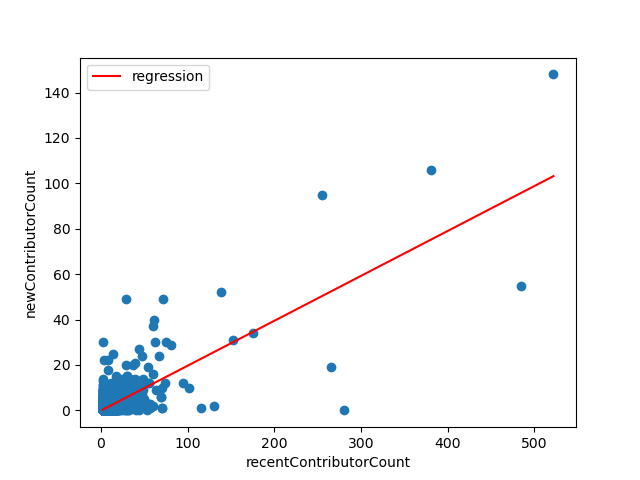
\includegraphics[width=\textwidth]{experiment/data_analysis/recentContributorCountRegression_linearScale.png}
        \caption{Échelle linéaire}
    \end{subfigure}%
    \begin{subfigure}[t]{0.5\textwidth}
        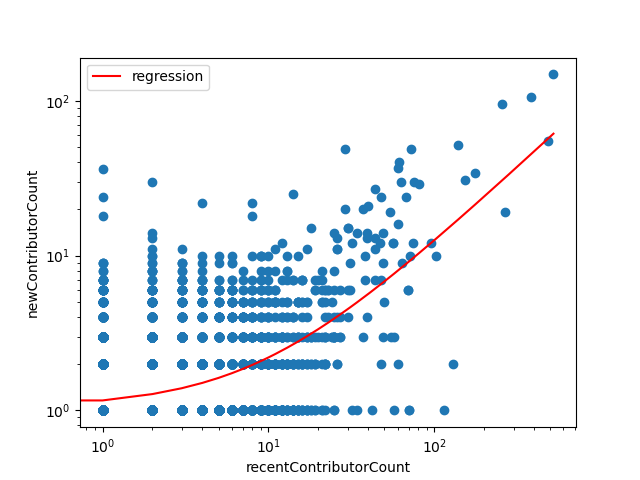
\includegraphics[width=\textwidth]{experiment/data_analysis/recentContributorCountRegression_logScale.png}
        \caption{Échelle logarithmique}
    \end{subfigure}

    $\mathit{newContributorCount} = \mathit{recentContributorCount} * 0.11540180 + 1.04427117$\\($r^2 = 0.28318792$)
    \caption{Nombre de nouveaux contributeurs en fonction du nombre de contributeurs récents uniques}
    \label{fig:contributorCount}
\end{figure}

\begin{figure}[ht]
    \centering
    \begin{subfigure}[t]{0.5\textwidth}
        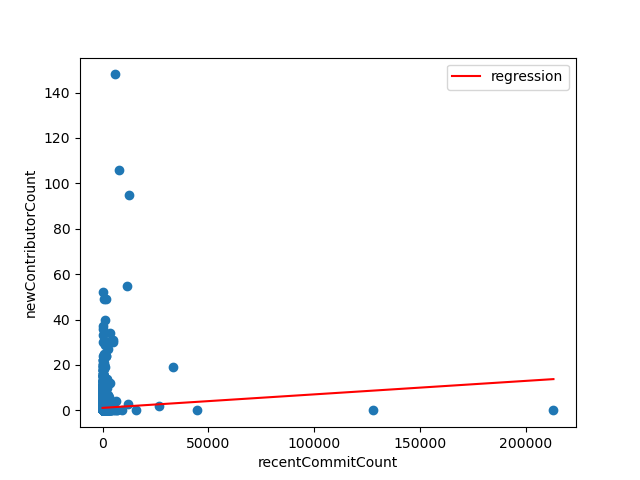
\includegraphics[width=\textwidth]{experiment/data_analysis/recentCommitCountRegression_linearScale.png}
        \caption{Échelle linéaire}
    \end{subfigure}%
    \begin{subfigure}[t]{0.5\textwidth}
        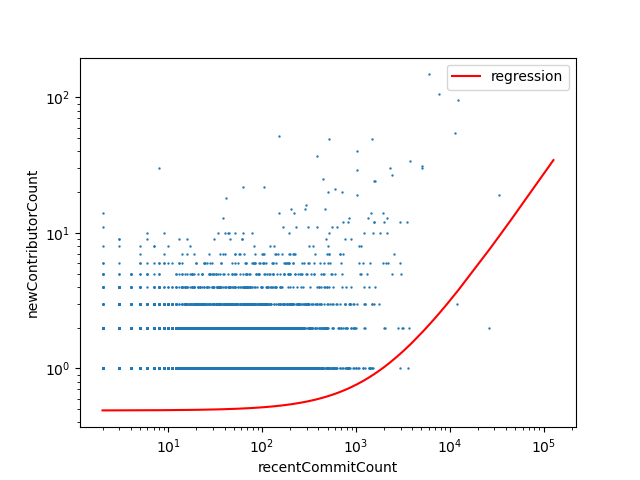
\includegraphics[width=\textwidth]{experiment/data_analysis/recentCommitCountRegression_logScale.png}
        \caption{Échelle logarithmique}
    \end{subfigure}

    $\mathit{newContributorCount} = \mathit{recentCommitCount} \times 0.00026672041 + 0.48979364$\\($r^2 = 0.12749825$)
    \caption{Nombre de nouveaux contributeurs en fonction du nombre de commits récents}
    \label{fig:commitCount}
\end{figure}

\pagelayout{margin}
